\section{Digital Teori}
\textit{Noget om denne section?}

Til dette projekt anvendes CY8CKIT-043 Programmable System on Chip (PSoC) 4 M-Series Prototyping Kit og programmet PSoC Creater i den digitale del til at opsamle det biologiske signal.\\
CY8CKIT-043 PSoC 4 M-Series Prototyping Kit er en prototyping platform, der indeholder tre mikroprocessorer: to Programmable System-on-Chips (PSoC) og en Programmable Radio on Chip (PRoC)% Advanced RISC\fxnote{REDUCED INSTRUCTION SET COMPUTER - RISK kan load/store og har pipelinable instructions, hbvilket betyder, at vi ikke behøver vente på, at en instruktion bliver færdig før vi starter med den næste. Fetch - decode - exicude, laver mere på samme tid. (kilde - slide første forelæsning)} Machines (ARM) mikroprocessorer
, hvilket ses på \figref{fig:PSoC}. Den første PSoC LP5 på mikrokontrolleren sidder på KitProg boardet og kan indeholde programmer, der kan indlæses på en computer ved hjælp af USB stikket. Den bruges til at programmere og debug softwaren på target boardet af mikrokontrolleren, hvorfor denne del kan knækkes af resten af stikket og fungere selvstændigt. Dette kræver dog, at softwaren først er programmeret på den anden mikroprocessorer, som er PSoC 4200M. Denne fungerer som hovedcomputeren, der programmeres på igennem c koden, og muliggøre eksempelvis høj-performans analog til digital konvertering (SAR ADC) . På bagsiden af mikrokontrolleren sidder en PRoC med Bluetooth Low Energy(BLE). Denne PRoC har ikke lige så mange muligheder for afbenyttelse i forhold til PRoC 4200M, da BLE optager meget plads, hvorfor der ikke er plads til meget andet. \citep{CYPRESS2016PSoC,Semiconductor2016}
\begin{figure}[H]
	\centering
	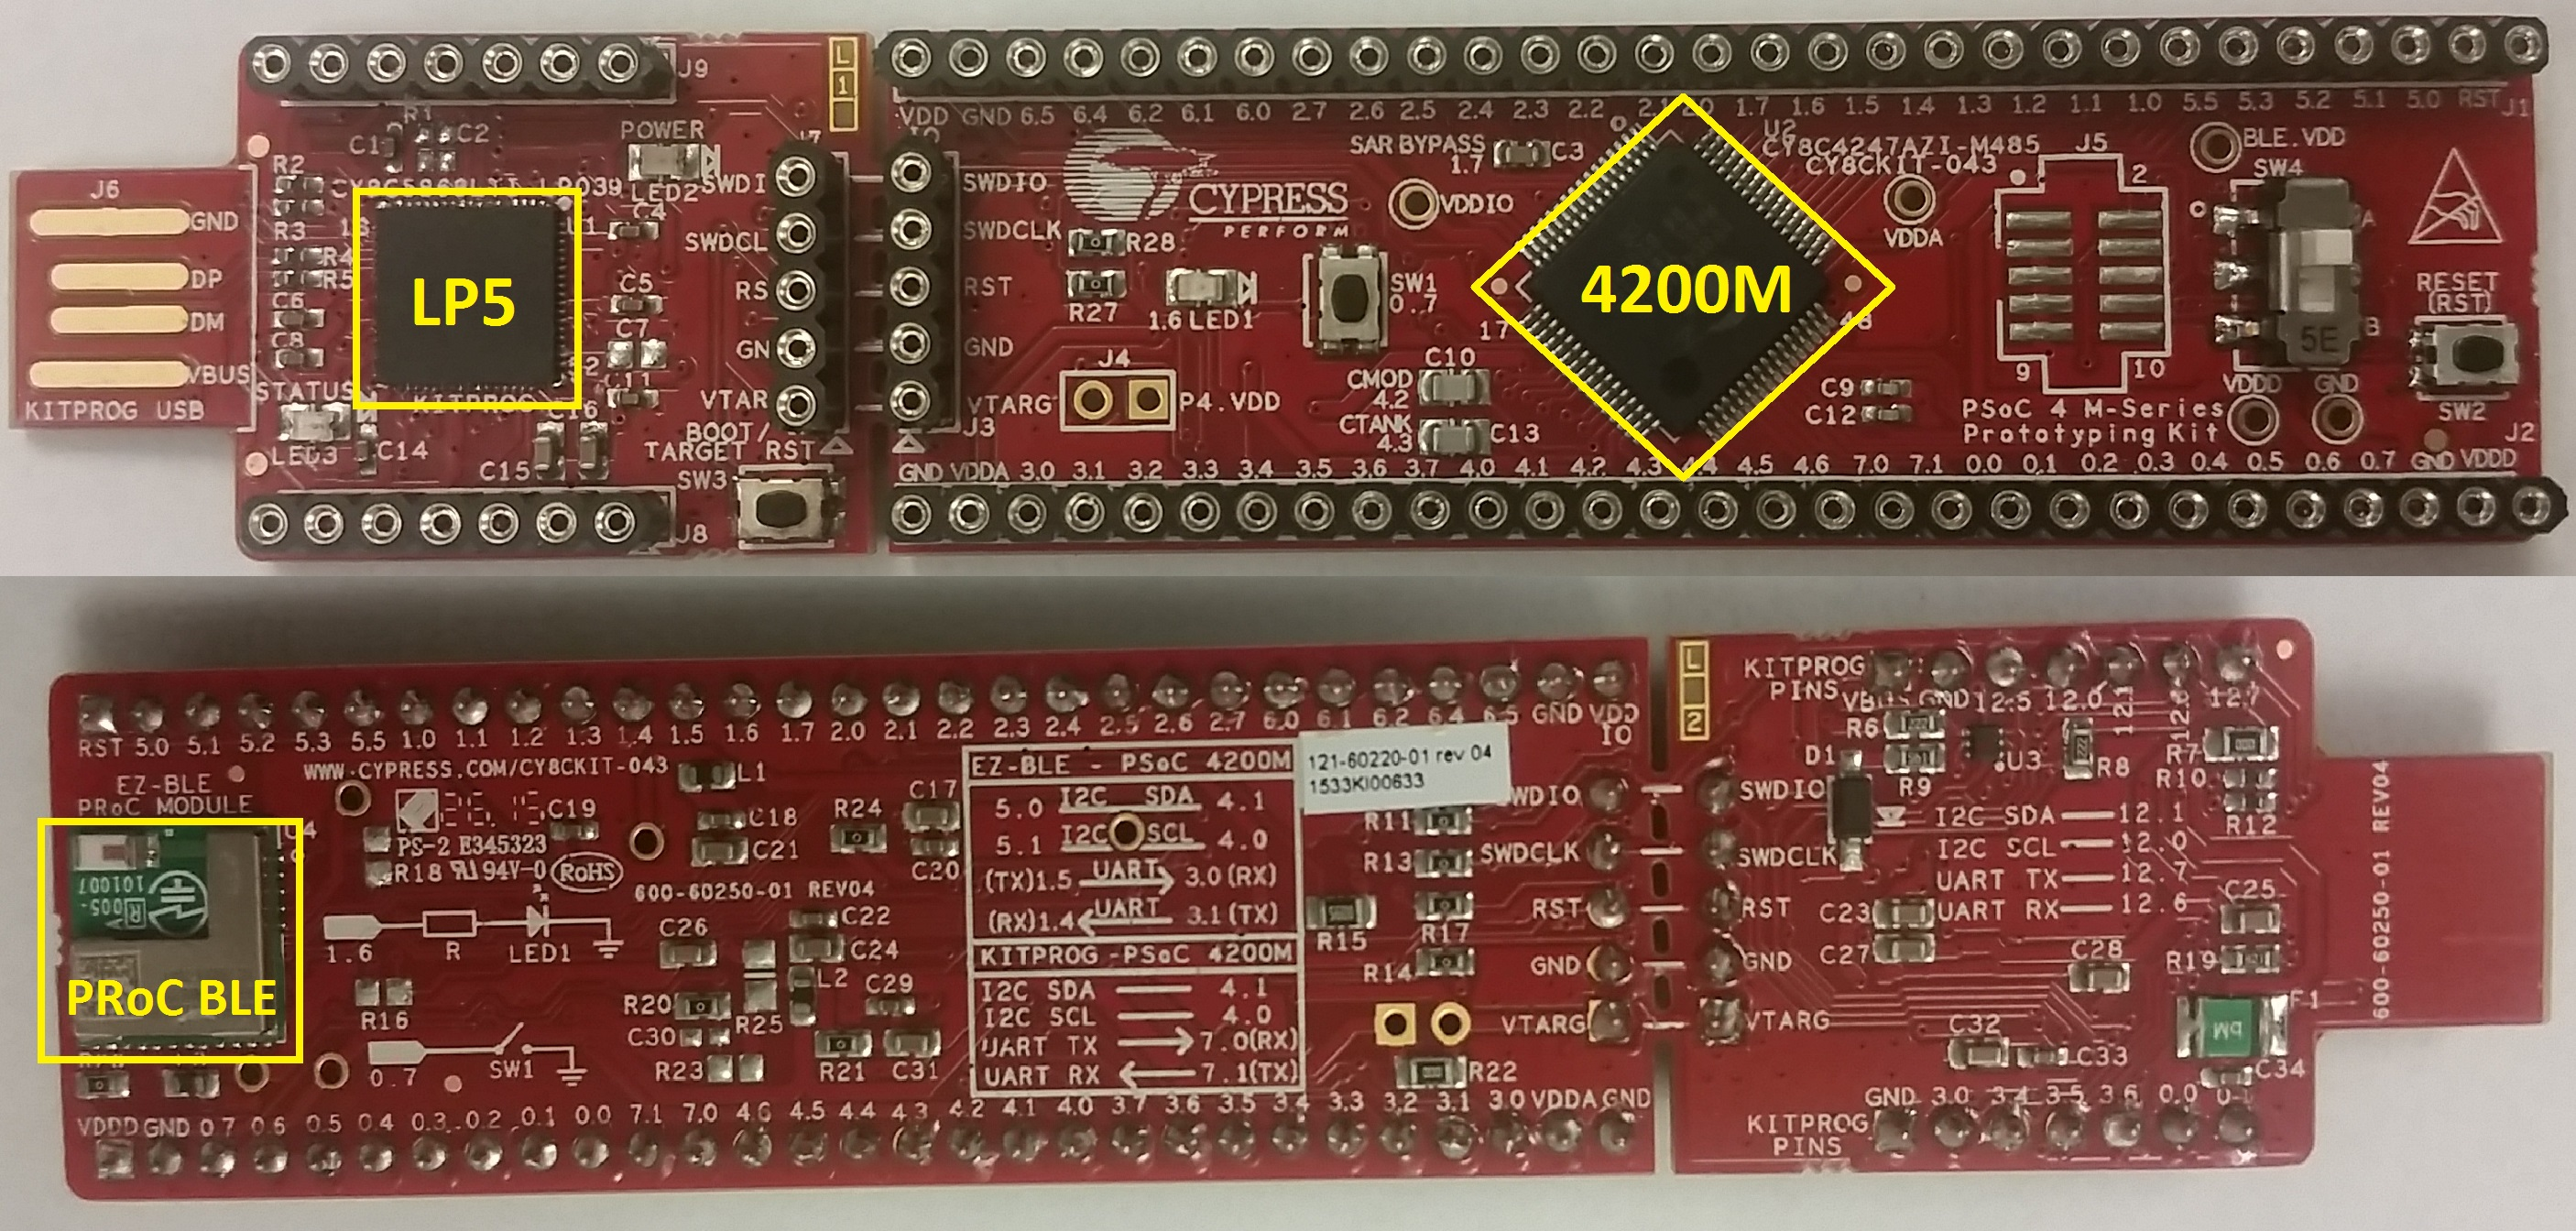
\includegraphics[scale=0.15]{figures/bProblemloesning/PSoC3.jpg}
	\caption{På figuren ses mikrokontrolleren CY8CKIT-043 PSoC 4 M-Series Prototyping Kit foran og bagpå. På forsiden findes to PSoC og på bagsiden findes PRoC, som alle er tydeliggjort med gul markering og navngivning. Mikrokontrolleren kan knækkes over i to: KipProg board med USB stik og target board med hovedchippen PSoC 4200M\fxnote{Navnene er fundet nederst på side 26 i manualen}. PRoC'en er ikke påmonteret som standart fra Cypress, hvorfor denne er blevet loddet manuelt på efterfølgende. Kontakten helt til højre på forsiden af target boardet, som også er loddet manuelt på efterfølgende, skal trykkes ned for, at PRoC programmeres på istedet for PSoC 4200M. \citep{CYPRESS2016PSoC,Semiconductor2016}}
	\label{fig:PSoC}
\end{figure}
Når data skal opsamles, skal to CY8CKIT-043 PSoC 4 M-Series Prototyping Kit benyttes. Én skal placeres på personen og opsamle data, som skal sendes til en anden mikrokontroller, der er koblet til en computer via USB. Dette kan lade sig gøre, da mikrokontrolleren har Inter-Integrated Circuit (I$^{2}$C) interface. I$^{2}$C er en computerbus dataprotokol, hvilket gør det muligt for de to mikrokontrollere at opføre sig som master eller slave. Rollen i kredsen bestemmes igennem softwaren. Masteren kontrollerer I$^{2}$C bussen og sender kommandoer til slaven. Både master og slave kan sende og modtage data, men masteren kontrollerer, hvornår dette kan finde sted. Det er muligt med I$^{2}$C interface at lave flere slaver eller flere masters til slaverne. I dette tilfælde vil der være én slave og én master. Disse kan kommunikere ved hjælp af et virtuelt kabel, som skabes af BLE. \citep{Semiconductor2016,Sparkfun2016}\\
Mellem PSoC LP5 og PSoC 4200M samt mellem PSoC 4200M og PRoC findes blandt andet nogle serielle porte med to ledninger til at modtage data (RX) og sende data (TX). Disse tre mikroprocessorer kommunikerer altså ikke på samme måde, som to mikrokontrollere kommunikerer med hinanden. \citep{Semiconductor2016} \\
Mikrokontrolleren kræver en ekstern strømkilde for at kunne fungere. Igennem USB porten adapteres tilslutningen til 5V, men det er muligt at tilkoble en strømkilde til boardets lav-volt applikation, hvilket gør den trådløs. 3,3V til 5,5V tilsluttes VDD fra en reguleret forsyning, hvilket er yderst essentielt, da boardet ikke besidder en elektrostatisk afladnings beskyttelse (ESD). Hvis en ekstern strømforsyning til VDD er for ustabil eller af dårlig kvalitet, kan mikrokontrollerens kredsløb blive forstyrret og vil derved ikke fungere optimalt. \citep{Semiconductor2016}

Programmet PSoC Creater kan designe hardware og software til mikrokontrolleren. Herigennem bliver rekonfigurerbare analoge blokke og digital programmerbar logik kombineret\fxnote{kan den fysiske hardware opbygges digitalt}, hvorved softwaren kan tilpasses de fysiske komponenter direkte igennem kodedesign. Programmet indeholder forskellige komponenter og kodeeksempler, hvilket kan blive behjælpeligt under algoritmedesignet. \citep{Semiconductor2016} \\
Når mikrokontrolleren er tilsluttet computeren og debugger igennem PSoC Creater, kan matlab fungere som et grafisk bruger interface (GUI). Dette muliggør live visualisering af den data, som eksempelvis en master mikrokontroller modtager fra en slave mikrokontroller. \fxnote{Hvis der skal skrives mere til, så undersøg CPU'en mere i dybden ift. 4200M, skriv om , interrups, clocs, LPM - inspiration i Detektion af Diafragmatisk Udtrætning af bla. Johannes.}
%
%
% I pdf'en for mikrokontrolleren - se side 23
% Skrive om I2C
%
%Denne prototyping Kit platform er ved hjælp af en computer med aktiv bluetooth i stand til at sende og modtage trådløs data fra Y8CKIT-042-BLE Bluetooth® Low Energy (BLE) Pioneer Kit platformen, som indeholder en PRoC.
%CYPRESS2016BLE
%CYPRESS2016PSoC
%Semiconductor2016
%Semiconductor2016BLE